%%%%%%%%%%%%%%%%%%%%%%%%%%%%%%%%%%%%%%%%%%%%%%%%%%%%%%%%%%%%%%%%%%%%%
%  GNDEC Industrial Training Report -- TR-104
%  Department of Information Technology
%  Six Months Industrial Training
%  Project: MERN Smart Education Platform
%
%  SPECIFICATIONS (from format document):
%  Font   : Times New Roman, 12pt
%  Paper  : A4
%  Spacing: Double space
%  Margins: Left 3.5cm | Top 2.5cm | Right 1.25cm | Bottom 1.25cm
%  Page#  : Center of footer
%  Front  : Roman numerals (i, ii ...)
%  Body   : Arabic numerals starting at 1 from Chapter 1
%  Each chapter starts on a fresh page
%%%%%%%%%%%%%%%%%%%%%%%%%%%%%%%%%%%%%%%%%%%%%%%%%%%%%%%%%%%%%%%%%%%%%

\documentclass[12pt, a4paper, oneside]{report}

% ---------------------------------------------------------------
%  FONTS  --  True Times New Roman (newtx is the gold standard)
%  newtxtext = Times New Roman text font
%  newtxmath = matching Times math font
%  Both are metric-compatible with Microsoft Times New Roman.
%  If compiling with XeLaTeX/LuaLaTeX you can instead use:
%    \usepackage{fontspec}
%    \setmainfont{Times New Roman}
% ---------------------------------------------------------------
\usepackage[T1]{fontenc}
\usepackage[utf8]{inputenc}
\usepackage{newtxtext, newtxmath}  % Best Times New Roman in pdfLaTeX

% ---------------------------------------------------------------
%  MARGINS  (spec: left 3.5, top 2.5, right 1.25, bottom 1.25)
% ---------------------------------------------------------------
\usepackage[
  a4paper,
  left=3.5cm,
  right=1.25cm,
  top=2.5cm,
  bottom=1.25cm,
  % includehead,      % Include header in top margin
  includefoot       % Include footer in bottom margin
]{geometry}



% ---------------------------------------------------------------
%  CORE PACKAGES
% ---------------------------------------------------------------
\usepackage{setspace}          % \doublespacing
\usepackage{graphicx}          % \includegraphics
\usepackage{float}             % [H] placement
\usepackage{placeins}          % \FloatBarrier  -- keeps tables on same page
\usepackage{caption}           % caption styling
\usepackage{booktabs}          % professional table rules
\usepackage{array}             % column types
\usepackage{tabularx}          % auto-width columns
\usepackage{ragged2e}          % \justifying inside boxes
\usepackage{microtype}         % better text justification (reduces overfull \hbox)
\usepackage{parskip}           % space between paragraphs, no indent
\usepackage{enumitem}          % list control
\usepackage{xcolor}            % colours
\usepackage{listings}          % code blocks
\usepackage{pgfgantt}          % Gantt chart
\usepackage{tikz}              % flowcharts / diagrams
\usetikzlibrary{shapes.geometric, arrows.meta, positioning, calc, fit}
\usepackage{pdflscape}         % landscape pages
\usepackage{fancyhdr}          % header/footer
\usepackage{tocloft}           % TOC / LOF / LOT
\usepackage{titlesec}          % chapter & section title format
\usepackage{amsmath}
\usepackage{url}
\usepackage[
  colorlinks = true,
  linkcolor  = black,
  citecolor  = black,
  urlcolor   = blue,
  pdftitle   = {MERN Smart Education Platform -- TR-104},
  pdfauthor  = {Jay Jaisswal}
]{hyperref}

% ---------------------------------------------------------------
%  GLOBAL SPACING
% ---------------------------------------------------------------
\doublespacing                 % double-space throughout
\setlength{\parindent}{0pt}   % no paragraph indent (parskip handles gaps)

% ---------------------------------------------------------------
%  JUSTIFICATION -- prevent ragged-right in double-spaced mode
% ---------------------------------------------------------------
\emergencystretch=1.5em        % allow slight stretch before overfull box

% ---------------------------------------------------------------
%  PAGE STYLE  -- plain header, centred page number in footer
% ---------------------------------------------------------------
\pagestyle{fancy}
\fancyhf{}
\renewcommand{\headrulewidth}{0pt}
\fancyfoot[C]{\thepage}

% Make chapter-opening pages also use fancy (not plain)
\fancypagestyle{plain}{%
  \fancyhf{}
  \renewcommand{\headrulewidth}{0pt}
  \fancyfoot[C]{\thepage}
}

% ---------------------------------------------------------------
%  CHAPTER TITLE FORMAT
%  Spec says 12pt body; chapter headings should be bold & clearly
%  larger -- 16pt bold centred is standard for such reports.
% ---------------------------------------------------------------
\titleformat{\chapter}[display]
  {\normalfont\fontsize{16}{19}\selectfont\bfseries\centering}
  {Chapter\ \thechapter}
  {8pt}
  {\fontsize{16}{19}\selectfont\bfseries}
\titlespacing*{\chapter}{0pt}{-35pt}{24pt}
% ---------------------------------------------------------------
%  FIX FOR TOC, LOF, LOT TOP MARGIN SPACING & LEFT ALIGNMENT
% ---------------------------------------------------------------
\usepackage{tocloft} 

% Adjust the top spacing (pulls titles up by exactly 35pt to match chapters)
\setlength{\cftbeforetoctitleskip}{-35pt}
\setlength{\cftbeforeloftitleskip}{-35pt}
\setlength{\cftbeforelottitleskip}{-35pt}

% Set the bottom spacing after titles before content starts
\setlength{\cftaftertoctitleskip}{24pt}
\setlength{\cftafterloftitleskip}{24pt}
\setlength{\cftafterlottitleskip}{24pt}

% Enforce left alignment, 16pt font size, and 19pt baseline
\renewcommand{\cfttoctitlefont}{\normalfont\fontsize{16}{19}\selectfont\bfseries}
\renewcommand{\cftaftertoctitle}{}

\renewcommand{\cftloftitlefont}{\normalfont\fontsize{16}{19}\selectfont\bfseries}
\renewcommand{\cftafterloftitle}{}

\renewcommand{\cftlottitlefont}{\normalfont\fontsize{16}{19}\selectfont\bfseries}
\renewcommand{\cftafterlottitle}{}
% Section: 14pt bold
\titleformat{\section}
  {\normalfont\fontsize{14}{17}\selectfont\bfseries}
  {\thesection}{1em}{}
\titlespacing*{\section}{0pt}{12pt}{6pt}

% Subsection: 13pt bold
\titleformat{\subsection}
  {\normalfont\fontsize{13}{16}\selectfont\bfseries}
  {\thesubsection}{1em}{}
\titlespacing*{\subsection}{0pt}{10pt}{4pt}

% Subsubsection: 12pt bold
\titleformat{\subsubsection}
  {\normalfont\fontsize{12}{15}\selectfont\bfseries}
  {\thesubsubsection}{1em}{}
\titlespacing*{\subsubsection}{0pt}{8pt}{4pt}

% ---------------------------------------------------------------
%  CAPTION RULES (spec: Fig caption BOTTOM, Table caption TOP)
% ---------------------------------------------------------------
\captionsetup[figure]{position=below, font=normalsize, labelfont=bf}
\captionsetup[table] {position=above, font=normalsize, labelfont=bf}

% ---------------------------------------------------------------
%  TOC depth
% ---------------------------------------------------------------
\setcounter{tocdepth}{3}
\setcounter{secnumdepth}{3}

% ---------------------------------------------------------------
%  CODE LISTING STYLE
% ---------------------------------------------------------------
\lstset{
  basicstyle   = \small\ttfamily,
  breaklines   = true,
  frame        = single,
  numbers      = left,
  numberstyle  = \tiny\color{gray},
  keywordstyle = \color{blue}\bfseries,
  commentstyle = \color{gray}\itshape,
  stringstyle  = \color{red},
  tabsize      = 2,
  showstringspaces = false
}

% ---------------------------------------------------------------
%  TIKZ STYLES  (used throughout for diagrams)
% ---------------------------------------------------------------
\tikzset{
  startstop/.style = {
    rectangle, rounded corners=6pt, draw=black, thick,
    fill=red!15, minimum width=3.2cm, minimum height=0.85cm,
    text centered, font=\small
  },
  process/.style = {
    rectangle, draw=black, thick,
    fill=blue!10, minimum width=3.8cm, minimum height=0.85cm,
    text centered, font=\small
  },
  decision/.style = {
    diamond, draw=black, thick, fill=green!12,
    minimum width=3.5cm, minimum height=1.1cm,
    text centered, font=\small, aspect=2.2
  },
  entity/.style = {
    rectangle, draw=black, thick,
    fill=gray!12, minimum width=2.5cm, minimum height=0.8cm,
    text centered, font=\small
  },
  dstore/.style = {
    rectangle, draw=black, thick,
    fill=yellow!20, minimum width=2.8cm, minimum height=0.8cm,
    text centered, font=\small
  },
  myarrow/.style = {-{Stealth[length=6pt]}, thick},
  dasharrow/.style = {-{Stealth[length=6pt]}, dashed}
}

%%%%%%%%%%%%%%%%%%%%%%%%%%%%%%%%%%%%%%%%%%%%%%%%%%%%%%%%%%%%%%%%%%%%%
\begin{document}

% ===============================================================
%  FRONT MATTER  -- Roman numerals
% ===============================================================
\pagenumbering{roman}

% ==============================================================
%  OUTER COVER  (title page -- no page number printed)
% ==============================================================
% ==============================================================
%  OUTER COVER  (title page -- no page number printed)
% ==============================================================
\begin{titlepage}
\thispagestyle{empty}
\begin{singlespace}
\begin{center}

% Pulled up tightly to match your 2.5cm margin requirements
\vspace*{-0.5cm} 

{\fontsize{24}{28}\selectfont\bfseries
    PADHO INDIA: SMART EDUCATIONAL\\[0.3cm] PLATFORM\par}\\[1.4cm]

{\fontsize{14}{17}\selectfont\bfseries REPORT}\\[0.8cm]

{\fontsize{12}{15}\selectfont
SUBMITTED IN PARTIAL FULFILLMENT OF THE REQUIREMENT FOR}\\[0.4cm]
{\fontsize{12}{15}\selectfont\bfseries Six Months Industrial Training (TR-104)}\\[0.8cm]

{\fontsize{12}{15}\selectfont at}\\[0.4cm]

{\fontsize{14}{17}\selectfont\bfseries Accelor Microsystems}\\[0.4cm]
{\fontsize{12}{15}\selectfont (from January to June)}\\[1.4cm]

{\fontsize{12}{15}\selectfont\bfseries SUBMITTED BY}\\[0.5cm]

{\fontsize{14}{17}\selectfont\bfseries Jay Kumar}\\[0.3cm]
{\fontsize{12}{15}\selectfont Branch: Information Technology}\\[0.2cm]
{\fontsize{12}{15}\selectfont Univ. Roll No.: 2203844}\\[0.2cm]
{\fontsize{12}{15}\selectfont Session: 2024--2025}\\[1.8cm] % Fixed spacing instead of elastic \vfill

% Logo section now flows naturally with the rest of the text
\includegraphics[width=3cm]{gndeclogo.png}\\[16pt]

{\fontsize{14}{17}\selectfont\bfseries
Department of Information Technology\\[0.4cm]
GURU NANAK DEV ENGINEERING COLLEGE\\[0.3cm]
LUDHIANA, INDIA}

\end{center}
\end{singlespace}
\end{titlepage}
% ==============================================================
%  INNER TITLE PAGE
% ==============================================================
% \newpage
% \thispagestyle{empty}
% \begin{center}

% \vspace*{0.8cm}
% {\fontsize{16}{20}\selectfont\bfseries
% MERN SMART EDUCATION PLATFORM}\\[1.2cm]

% {\fontsize{14}{17}\selectfont\bfseries REPORT}\\[0.6cm]

% {\fontsize{12}{15}\selectfont
% SUBMITTED IN PARTIAL FULFILLMENT OF THE REQUIREMENT FOR}\\[0.3cm]
% {\fontsize{12}{15}\selectfont\bfseries Six Months Industrial Training (TR-104)}\\[0.6cm]

% {\fontsize{12}{15}\selectfont at}\\[0.4cm]

% {\fontsize{14}{17}\selectfont\bfseries [Company Name, City]}\\[0.4cm]
% {\fontsize{12}{15}\selectfont (from \underline{\hspace{3.5cm}} to \underline{\hspace{3.5cm}})}\\[1.0cm]

% {\fontsize{12}{15}\selectfont\bfseries SUBMITTED BY}\\[0.5cm]

% {\fontsize{14}{17}\selectfont\bfseries Jay Jaisswal}\\[0.3cm]
% {\fontsize{12}{15}\selectfont Branch: Information Technology}\\[0.2cm]
% {\fontsize{12}{15}\selectfont Univ. Roll No.: \underline{\hspace{4.5cm}}}

% \vfill

% {\fontsize{14}{17}\selectfont\bfseries
% Department of Information Technology\\[0.4cm]
% GURU NANAK DEV ENGINEERING COLLEGE\\[0.3cm]
% LUDHIANA, INDIA}

% \end{center}

% ==============================================================
%  COMPANY CERTIFICATE
% ==============================================================
\newpage
% 1. Turn off page numbers for chapters in the TOC
\addtocontents{toc}{\protect\cftpagenumsoff{\textbf{\textit Certificate}}}




\thispagestyle{fancy}
\begin{center}
{\fontsize{14}{17}\selectfont\bfseries [COMPANY LETTER HEAD]}\\[1.5cm]
{\fontsize{14}{17}\selectfont\bfseries TO WHOM IT MAY CONCERN}
\end{center}

\vspace{0.8cm}

I hereby certify that \textbf{Jay Kumar}, University Roll No.\ \underline{\hspace{3cm}} of Guru Nanak Dev Engineering College, Ludhiana, has undergone Six Months Industrial Training from \underline{\hspace{3cm}} to \underline{\hspace{3cm}} at our organization to fulfill the requirements for the award of degree of B.Tech.\ in Information Technology. He has worked on the \textbf{MERN Smart Education Platform} project during the training under the supervision of \underline{\hspace{4cm}}. During his/her tenure with us we found him/her sincere and hard working. Wishing him/her great success in the future.

\vspace{3cm}

\begin{flushright}
Signature of the Supervisor(s)\\[0.5cm]
(Seal of Organization)
\end{flushright}

% ==============================================================
%  STUDENT'S DECLARATION  -- Page i
% ==============================================================
\newpage
\setcounter{page}{1}
\addcontentsline{toc}{chapter}{\textit{Student's Declaration}}
\begin{center}
{\fontsize{16}{19}\selectfont\bfseries Student's Declaration}
\end{center}

\vspace{0.4cm}

I hereby certify that the work which is being presented in this training report with the project entitled \textbf{``Padho India : MERN Smart Education Platform''} by \textbf{Jay Kumar}, University Roll No.\ \underline{\hspace{3cm}} in partial fulfillment of requirements for the award of degree of B.Tech.\ (Information Technology) submitted in the Department of Information Technology at GURU NANAK DEV ENGINEERING COLLEGE, LUDHIANA under I.K.\ GUJRAL PUNJAB TECHNICAL UNIVERSITY is an authentic record of my own work carried out under the supervision of \underline{\hspace{4cm}}, \underline{\hspace{3.5cm}} (Designation) of \underline{\hspace{3.5cm}} (Company Name). The matter presented has not been submitted by me in any other University/Institute for the award of B.Tech.\ Degree.

\vfill % Dynamically distributes remaining space safely

\noindent Student Name:\quad \underline{\hspace{6cm}}\\[6pt]
\noindent Univ. Roll No.:\quad \underline{\hspace{6cm}}\\[6pt]
\noindent (Signature of Student) \hfill Date: \underline{\hspace{3cm}}

\vfill % Dynamically distributes remaining space safely

\noindent This is to certify that the above statement made by the candidate is correct to the best of my knowledge.

\vfill % Dynamically distributes remaining space safely

\noindent Signature of Internal Examiner \hfill Date: \underline{\hspace{3cm}}

\vfill % Dynamically distributes remaining space safely

\noindent The External Viva-Voce Examination of the student has been held on \underline{\hspace{3cm}}.

\vfill % Dynamically distributes remaining space safely

\noindent Signature of External Examiner \hfill Signature of HOD
% ==============================================================
%  ABSTRACT  -- Page ii
% ==============================================================
\newpage
\addcontentsline{toc}{chapter}{\textit{Abstract}}
\begin{center}
{\fontsize{16}{19}\selectfont\bfseries Abstract}
\end{center}

\vspace{0.5cm}

The MERN Smart Education Platform is a full-stack web application developed using the MERN stack (MongoDB, Express.js, React.js, and Node.js) aimed at modernizing the delivery and management of educational content. The platform provides a comprehensive environment for students, instructors, and administrators to interact in a single digital ecosystem. It supports features including user authentication with JWT-based security, course creation and enrollment, real-time progress tracking, lecture streaming, quiz management, and dashboard analytics.

The system addresses key shortcomings of traditional classroom-based learning by offering a scalable and responsive interface that functions across all devices. The backend RESTful API is built with Node.js and Express.js, and data is persisted using MongoDB through the Mongoose ODM. The frontend is developed using React.js with Redux for state management and Tailwind CSS for responsive design.

During the six months of industrial training, the complete software development lifecycle (SDLC) was followed --- from requirement gathering and feasibility analysis, through system design using UML and data flow diagrams, to implementation, testing, and deployment. The system was validated using manual test cases and Postman for API testing. The platform demonstrates a practical application of modern web development technologies in the education domain and forms the foundation for scalable EdTech solutions.

% ==============================================================
%  ACKNOWLEDGEMENT  -- Page iii
% ==============================================================
\newpage
\addcontentsline{toc}{chapter}{\textit{Acknowledgement}}
\begin{center}
{\fontsize{16}{19}\selectfont\bfseries Acknowledgement}
\end{center}

\vspace{0.5cm}

I am highly grateful to the Principal, Guru Nanak Dev Engineering College (GNDEC), Ludhiana, for providing this opportunity to carry out Six Months Industrial Training at \underline{\hspace{4cm}}.

The constant guidance and encouragement received from the Head of the Department, Information Technology, GNDEC Ludhiana has been of great help during the training and project work and is acknowledged with reverential thanks.

I would like to express a deep sense of gratitude and thanks profusely to \underline{\hspace{3cm}}, Director/CEO of \underline{\hspace{3cm}}. Without the wise counsel and able guidance, it would have been impossible to complete the report in this manner.

The help rendered by \underline{\hspace{3cm}}, Designation (\underline{\hspace{2.5cm}} Department) for guidance and experimentation is greatly acknowledged.

I express gratitude to other faculty members of the Information Technology Department of GNDEC for their intellectual support throughout the course of this work.

Finally, I am indebted to all whosoever have contributed to this report work and provided a friendly environment during the training at \underline{\hspace{3cm}}.

\vspace{2.5cm}

\begin{flushright}
\textbf{Jay Kumar}\\
Univ.\ Roll No.: 2203844 {\hspace{3.5cm}}
\end{flushright}

% ==============================================================
%  LIST OF FIGURES  -- Page iv
% ==============================================================
\newpage
\addcontentsline{toc}{chapter}{\textit{List of Figures}}
\listoffigures

% ==============================================================
%  LIST OF TABLES  -- Page v
% ==============================================================
\newpage
\addcontentsline{toc}{chapter}{\textit{List of Tables}}
\listoftables

% ==============================================================
%  TABLE OF CONTENTS  -- Page vi
% ==============================================================
\newpage
\addcontentsline{toc}{chapter}{\textit{Table of Contents  }}
\tableofcontents

% ===============================================================
%  BODY  -- Arabic numerals from Chapter 1 onwards
% ===============================================================
\newpage
\pagenumbering{arabic}
\setcounter{page}{1}

%%%%%%%%%%%%%%%%%%%%%%%%%%%%%%%%%%%%%%%%%%%%%%%%%%%%%%%%%%%%%%%%%%%%%
%  CHAPTER 1: INTRODUCTION
%%%%%%%%%%%%%%%%%%%%%%%%%%%%%%%%%%%%%%%%%%%%%%%%%%%%%%%%%%%%%%%%%%%%%
\chapter{Introduction}

\section{Introduction to Organization}

Accelor Microsystems, located in the prominent IT hub of Mohali (Sahibzada Ajit Singh Nagar), Punjab, is a leading technology solutions provider specializing in full-stack web engineering, custom embedded systems, and enterprise cloud architectures. Established with a vision to bridge the gap between complex industrial engineering requirements and modern software capabilities, the organization has consistently delivered high-performance digital solutions to a diverse global clientele. 

Operating from its state-of-the-art facility in Mohali, Accelor Microsystems serves as a hub for innovation, research, and collaborative development. The company specializes in the development of robust web applications, data-driven enterprise resource planning (ERP) platforms, and real-time analytical tools. By maintaining a sharp focus on modern, scalable development stacks—particularly the MongoDB, Express.js, React.js, and Node.js (MERN) ecosystem—the organization empowers businesses to execute secure digital transformations.

\subsection{Historical Background and Evolution}

Accelor Microsystems was founded by a core team of passionate systems engineers and software architects who recognized the impending industry shift toward decoupled web architectures and real-time distributed computing. In its initial years, the company focused on providing localized automation software and basic web hosting infrastructures for engineering enterprises.

As the global IT landscape transitioned from monolithic architectures to cloud-native, asynchronous web systems, Accelor Microsystems rapidly scaled its engineering operations. The firm invested heavily in building dedicated labs for open-source JavaScript engineering, cloud multi-tenancy testing, and agile development pipelines. Today, the Mohali facility stands as a premier technical delivery center, recognized for cultivating high-caliber engineering talent and delivering highly responsive applications that maintain sub-second latency targets under heavy network loads.

\subsection{Vision and Mission Statements}

The operational philosophy of Accelor Microsystems is governed by its corporate core values, which emphasize technological integrity, architectural scalability, and localized engineering innovation.

\textbf{Corporate Vision:} \\
To be a globally recognized center of engineering excellence that shapes the future of enterprise software solutions, fostering an ecosystem where complex industrial workflows are simplified through highly intuitive, open-source web technologies.

\textbf{Corporate Mission:}
\begin{itemize}[leftmargin=1.5cm, itemsep=4pt]
    \item To engineer secure, scalable, and highly available full-stack software architectures that drive measurable business outcomes for clients.
    \item To maintain an industry-aligned research environment that actively adapts to emerging technological paradigm shifts, such as serverless computing, reactive UI state machines, and non-blocking I/O microservices.
    \item To mentor and cultivate the next generation of software engineers by exposing them to rigorous Agile software development lifecycles (SDLC) and modern engineering benchmarks.
\end{itemize}

\subsection{Core Services and Product Portfolios}

Accelor Microsystems divides its operational workflows into three highly cohesive engineering divisions, ensuring specialized focus across different tech domains:

\subsubsection{1. Full-Stack Web Application Development}
This division forms the core software execution arm of the company. It specializes in designing modern client-side architectures utilizing React.js, coupled with high-throughput backend computing nodes powered by Node.js and Express.js. The team structurally implements Single Page Application (SPA) paradigms, global state containers (Redux/Context API), and RESTful API integrations with rigid input validation layers.

\subsubsection{2. Enterprise Cloud and Database Solutions}
The cloud division focuses on designing structured and unstructured cloud database storage frameworks, primarily utilizing MongoDB Atlas and distributed relational clusters. Services include schema design, query optimization, indexing strategies, and setting up secure connection pooling systems using cross-environment variables.

\subsubsection{3. Industrial Automation and Micro-Services}
Bridging software with hardware constraints, this subset of the company designs lightweight communication interfaces and protocols that allow microservices to interact smoothly with external distributed cloud layers, making it highly relevant for modern Internet-of-Things (IoT) ecosystems.

\subsection{Organizational Structure}

The administrative and technical governance at Accelor Microsystems follows a modular hierarchical matrix designed to streamline cross-departmental communication and accelerate Agile sprint tracking. The structural breakdown of the technical division is outlined in Figure 1.1 below.

\begin{figure}[H]
\centering
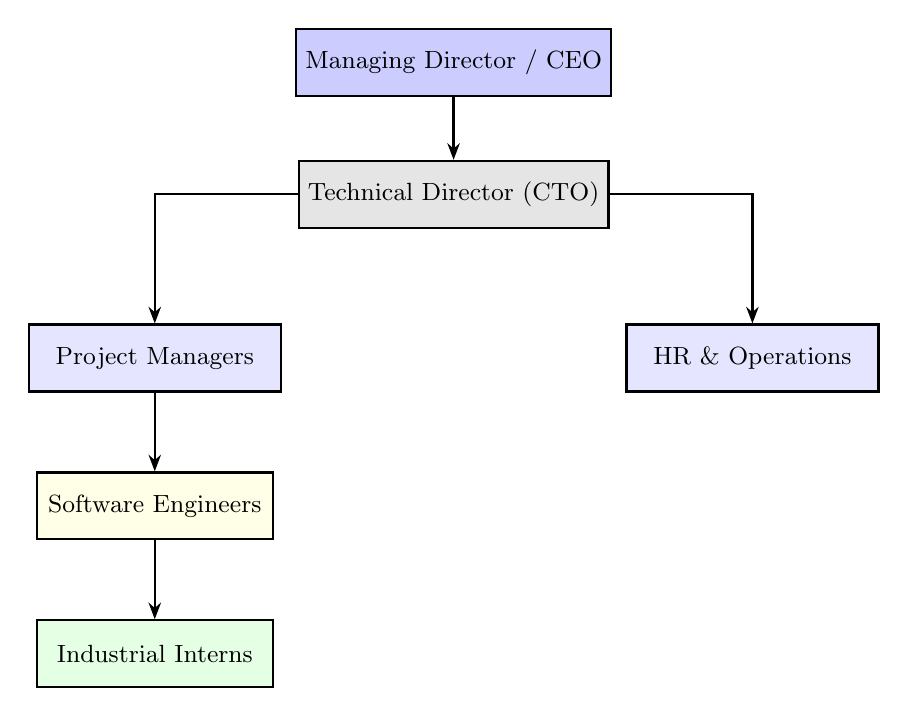
\begin{tikzpicture}[node distance=1.2cm and 1.5cm, auto]
  % Nodes
  \node[process, fill=blue!20, minimum width=4cm] (ceo) {Managing Director / CEO};
  \node[process, fill=gray!20, below=0.8cm of ceo, minimum width=3.5cm] (cto) {Technical Director (CTO)};
  
  \node[process, below left=1.2cm and 0.2cm of cto, minimum width=3.2cm] (pm) {Project Managers};
  \node[process, below right=1.2cm and 0.2cm of cto, minimum width=3.2cm] (hr) {HR \& Operations};
  
  \node[process, below=1.0cm of pm, minimum width=3cm, fill=yellow!10] (se) {Software Engineers};
  \node[process, below=1.0cm of se, minimum width=3cm, fill=green!10] (interns) {Industrial Interns};

  % Connections
  \draw[myarrow] (ceo) -- (cto);
  \draw[myarrow] (cto) -| (pm);
  \draw[myarrow] (cto) -| (hr);
  \draw[myarrow] (pm) -- (se);
  \draw[myarrow] (se) -- (interns);
\end{tikzpicture}
\caption{Organizational Hierarchy and Technical Reporting Workflow}
\label{fig:org_structure}
\end{figure}

The flat operational structure within the engineering blocks ensures that development teams, consisting of senior software engineers, QA specialists, and industrial interns, can collaborate dynamically during two-week Scrum review phases. This structural alignment allows the organization to maintain strict delivery schedules while providing an exceptional learning curve for engineering trainees working on live project modules.

% Uncomment to add company image:
%\begin{figure}[H]
%  \centering
%  \includegraphics[width=0.5\textwidth]{company_logo.png}
%  \caption{Logo of the Training Organization}
%  \label{fig:org_logo}
%\end{figure}

\section{Introduction to Project}

The MERN Smart Education Platform is a web-based application designed to facilitate online learning and course management. It brings together students, educators, and administrators onto a single unified platform. The project leverages the MERN stack --- MongoDB for database management, Express.js as the web framework, React.js for the frontend user interface, and Node.js as the runtime environment on the server side.

The platform enables instructors to create and publish courses with video lectures, quizzes, and assignments. Students can browse courses, enroll, and track their progress in real time. Administrators manage users, content, and overall system health through a dedicated dashboard.

\section{Project Category}

This project falls under the category of \textbf{Internet-Based Application Development}. It is a cloud-deployable, browser-accessible web application developed using modern JavaScript technologies and a RESTful API architecture.

\section{Objectives}

The primary objectives of the MERN Smart Education Platform are listed below.

\begin{itemize}[leftmargin=1.5cm, itemsep=2pt]
  \item To provide a scalable and user-friendly online Learning Management System (LMS).
  \item To enable instructors to create, manage, and publish course content with ease.
  \item To allow students to enroll in courses, view lectures, Practice MCQs.
  \item To implement secure user authentication and role-based access control.
  \item To design a fully responsive interface accessible on both desktop and mobile devices.
  \item To persist data reliably using MongoDB and expose it through RESTful APIs.
\end{itemize}

\section{Problem Formulation}

Traditional education systems are constrained by geographic location, fixed schedules, and limited scalability. Students in remote or underserved areas lack access to quality educational resources. Existing commercial platforms are often expensive and offer limited customization for smaller institutions. There is a clear need for an open, full-stack educational platform that demonstrates modern web development practices while solving real-world access problems in the domain of education.

\section{Identification / Recognition of Need}

With the rapid digitization of education following the COVID-19 pandemic, demand for robust Learning Management Systems has surged significantly. Institutions require platforms that are cost-effective, easy to deploy, and feature-rich. The MERN Smart Education Platform addresses this need by providing a customizable, open-source alternative with a modern user interface, real-time progress tracking, and secure authentication mechanisms.

\section{Existing System}

Existing e-learning platforms such as Coursera, Udemy, and Moodle provide online course delivery. However, these platforms are either fully proprietary, expensive to license, or complex to self-host and customize. They offer limited flexibility for small institutions and independent developers. Additionally, most existing systems do not provide accessible codebases for learning, modification, or academic study.

\section{Proposed System}

The proposed MERN Smart Education Platform is a self-hostable, full-stack web application with the following key characteristics.

\begin{itemize}[leftmargin=1.5cm, itemsep=2pt]
  \item Full MERN stack implementation for end-to-end JavaScript development.
  \item JWT-based authentication for secure login and session management.
  \item Role-based access control covering Student, Instructor, and Admin roles.
  \item RESTful API backend with proper error handling and middleware protection.
  \item Responsive React.js frontend with a modular component-based architecture.
  \item MongoDB for flexible, document-based data storage.
\end{itemize}

\section{Unique Features of the System}

\begin{itemize}[leftmargin=1.5cm, itemsep=2pt]
  \item \textbf{Unified JavaScript Stack:} JavaScript is used across the entire application --- frontend, backend, and database queries --- reducing context switching and simplifying development.
  \item \textbf{Real-Time Progress Tracking:} Students can monitor their course completion percentage lecture by lecture.
  \item \textbf{Instructor Dashboard:} A dedicated interface provides course analytics including enrollment count and performance data.
  \item \textbf{Secure Authentication:} JWT tokens stored in HTTP-only cookies protect against XSS attacks.
  \item \textbf{Modular Architecture:} Each feature is developed as a separate, independently testable module for easy future extension.
\end{itemize}

%%%%%%%%%%%%%%%%%%%%%%%%%%%%%%%%%%%%%%%%%%%%%%%%%%%%%%%%%%%%%%%%%%%%%
%  CHAPTER 2: REQUIREMENT ANALYSIS AND SYSTEM SPECIFICATION
%%%%%%%%%%%%%%%%%%%%%%%%%%%%%%%%%%%%%%%%%%%%%%%%%%%%%%%%%%%%%%%%%%%%%
\chapter{Requirement Analysis and System Specification}

\section{Feasibility Study}

\subsection{Technical Feasibility}

The platform is technically feasible as all technologies used are open-source and widely supported by large developer communities. Node.js and React.js are industry-standard, with extensive documentation and third-party library support. MongoDB Atlas provides free-tier cloud hosting suitable for development and small-scale production. The development environment requires only standard computing hardware with internet connectivity.

\subsection{Economical Feasibility}

The project uses entirely free and open-source tools. Deployment can be carried out on the free tiers of cloud platforms such as Render, Railway, or Vercel. No paid software licenses are required at any stage of development, making the project economically viable for educational institutions with limited budgets.

\subsection{Operational Feasibility}

The web-based nature of the platform means users require only a modern web browser for access. The interface is intuitive and modern, minimizing the training required for new users. All administrative tasks are accessible through a graphical dashboard, reducing operational complexity and the need for technical expertise among end users.

\section{Software Requirement Specification}

\subsection{Data Requirements}

The system manages the following core data entities.

\begin{itemize}[leftmargin=1.5cm, itemsep=2pt]
  \item \textbf{User:} Name, email, hashed password, role (student, instructor, or admin), profile image, and list of enrolled courses.
  \item \textbf{Course:} Title, description, instructor ID (reference), category, thumbnail, list of lectures, price, and enrolled student IDs.
  \item \textbf{Lecture:} Title, video URL or file path, duration, and parent course ID reference.
  \item \textbf{Progress:} User ID reference, course ID reference, list of completed lecture IDs, and completion percentage.
\end{itemize}

\subsection{Functional Requirements}

\begin{itemize}[leftmargin=1.5cm, itemsep=2pt]
  \item User registration and login using email and password.
  \item Role-based access control for Student, Instructor, and Admin roles.
  \item Instructors can create, edit, publish, and delete courses and lectures.
  \item Students can browse available courses, enroll, and view lecture content.
  \item Real-time progress tracking per course per student.
  \item Admin can view and manage all users and courses on the platform.
  \item Secure logout with session invalidation.
\end{itemize}

\subsection{Performance Requirements}

The system should handle concurrent requests from multiple users without degradation. API response time should remain under 500\,ms for all standard CRUD operations under normal load. The React frontend should achieve a Google Lighthouse performance score above 80.

\subsection{Dependability Requirement}

The system must maintain 99\% uptime during normal operation hours. MongoDB Atlas provides automatic failover and data redundancy at the database layer. React error boundaries are implemented on the frontend to prevent full-application crashes on component-level errors.

\subsection{Maintainability Requirement}

The backend follows the MVC (Model-View-Controller) architectural pattern, keeping business logic, data access, and routing clearly separated. React components are reusable, well-named, and organized by feature. All configuration values (database URIs, JWT secrets, port numbers) are stored in environment variables, making deployment and reconfiguration straightforward.

\subsection{Security Requirement}

\begin{itemize}[leftmargin=1.5cm, itemsep=2pt]
  \item User passwords are hashed using bcrypt with a salt factor of 10 before storage.
  \item JWT tokens are stored in HTTP-only cookies to mitigate XSS-based token theft.
  \item All protected API routes are guarded by authentication middleware.
  \item Input validation is performed on both the client side and the server side.
  \item Role checks are enforced at the controller level for all sensitive operations.
\end{itemize}

\subsection{Look and Feel Requirement}

The application features a modern, clean interface styled with Tailwind CSS. All pages follow a consistent layout including a top navigation bar, a collapsible sidebar for dashboard views, and a central content area. The design is fully responsive and adapts to screen widths from 320\,px (mobile) to 1920\,px (large desktop). The colour scheme uses a blue-and-white palette with contrast ratios that meet WCAG AA accessibility standards.

\section{Validation}

Input fields are validated on the client side using React-controlled form state and on the server side using the \texttt{express-validator} middleware. Mongoose schema validation enforces data type and required field constraints at the database layer, ensuring end-to-end data integrity.

\section{Expected Hurdles}

\begin{itemize}[leftmargin=1.5cm, itemsep=2pt]
  \item Managing shared state across deeply nested React components without excessive prop-drilling.
  \item Handling Cross-Origin Resource Sharing (CORS) mismatches between the frontend and backend during development.
  \item Implementing secure and efficient file uploads for video lecture content.
  \item Optimizing the delivery of large video files to prevent long buffering times for students.
\end{itemize}

\section{SDLC Model to be Used}

The project follows the \textbf{Agile SDLC model} with iterative two-week sprints. Each sprint had clearly defined user stories, acceptance criteria, and deliverables. This approach enabled continuous integration of feedback, early detection of issues, and incremental delivery of working modules throughout the training period.

%%%%%%%%%%%%%%%%%%%%%%%%%%%%%%%%%%%%%%%%%%%%%%%%%%%%%%%%%%%%%%%%%%%%%
%  CHAPTER 3: SYSTEM DESIGN
%%%%%%%%%%%%%%%%%%%%%%%%%%%%%%%%%%%%%%%%%%%%%%%%%%%%%%%%%%%%%%%%%%%%%
\chapter{System Design}

\section{Design Approach}

The system adopts an \textbf{Object-Oriented Design} approach on the backend, with Mongoose models representing the key domain entities. On the frontend, a \textbf{Component-Based Architecture} is used with React.js, where the UI is composed of self-contained, reusable components. The overall application structure follows the \textbf{MVC (Model-View-Controller)} pattern, cleanly separating data, business logic, and presentation.

\section{Detail Design}

The application is organized into three architectural layers.

\begin{itemize}[leftmargin=1.5cm, itemsep=2pt]
  \item \textbf{Presentation Layer:} A React.js Single Page Application (SPA) with Redux Toolkit for global state management and React Router for client-side navigation.
  \item \textbf{Business Logic Layer:} Express.js route handlers and controller functions that process requests, enforce business rules, and return structured responses.
  \item \textbf{Data Layer:} MongoDB collections accessed through the Mongoose ODM, with schemas defining structure and validation rules.
\end{itemize}

\section{System Design using Structured Analysis and Design Tools}

\subsection{Data Flow Diagram}

\subsubsection{Level 0 DFD (Context Diagram)}

\begin{figure}[H]
\centering
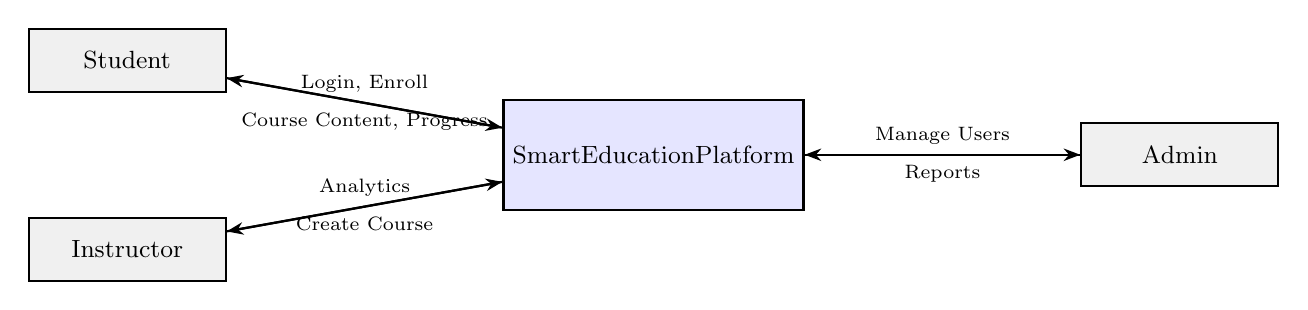
\begin{tikzpicture}[node distance=2.2cm]
  % Central process
  \node[process, minimum width=3.5cm, minimum height=1.4cm] (sys)
    {Smart\\Education\\Platform};
  % External entities
  \node[entity, left=3.5cm of sys, yshift= 1.2cm] (student)   {Student};
  \node[entity, left=3.5cm of sys, yshift=-1.2cm] (instructor){Instructor};
  \node[entity, right=3.5cm of sys]               (admin)     {Admin};
  % Arrows
  \draw[myarrow] (student)    -- node[above,font=\scriptsize]{Login, Enroll}    (sys);
  \draw[myarrow] (sys) -- node[below,font=\scriptsize]{Course Content, Progress} (student);
  \draw[myarrow] (instructor) -- node[below,font=\scriptsize]{Create Course}    (sys);
  \draw[myarrow] (sys) -- node[above,font=\scriptsize]{Analytics}               (instructor);
  \draw[myarrow] (admin)      -- node[above,font=\scriptsize]{Manage Users}     (sys);
  \draw[myarrow] (sys)        -- node[below,font=\scriptsize]{Reports}          (admin);
\end{tikzpicture}
\caption{Level 0 DFD -- Context Diagram of the Smart Education Platform}
\label{fig:dfd0}
\end{figure}

\subsubsection{Level 1 DFD}

\begin{figure}[H]
\centering
\begin{tikzpicture}[node distance=1.4cm and 2.5cm]
  % Row 1 -- Auth
  \node[entity]  (u1) {User};
  \node[process, right=2cm of u1] (p1) {P1: Auth\\Module};
  \node[dstore,  right=2cm of p1] (d1) {D1: Users};
  % Row 2 -- Course
  \node[entity,  below=1.5cm of u1] (u2) {Instructor};
  \node[process, right=2cm of u2]   (p2) {P2: Course\\Management};
  \node[dstore,  right=2cm of p2]   (d2) {D2: Courses};
  % Row 3 -- Progress
  % \node[entity,  below=1.5cm of u2] (u3) {Student};
  % \node[process, right=2cm of u3]   (p3) {P3: Progress\\Tracking};
  % \node[dstore,  right=2cm of p3]   (d3) {D3: Progress};
  % Arrows row 1
  \draw[myarrow] (u1) -- node[above,font=\scriptsize]{Credentials} (p1);
  \draw[myarrow] (p1) -- node[above,font=\scriptsize]{Store/Retrieve} (d1);
  % Arrows row 2
  \draw[myarrow] (u2) -- node[above,font=\scriptsize]{Course Data} (p2);
  \draw[myarrow] (p2) -- node[above,font=\scriptsize]{Read/Write} (d2);
  % Arrows row 3
  \draw[myarrow] (u3) -- node[above,font=\scriptsize]{View Lecture} (p3);
  % \draw[myarrow] (p3) -- node[above,font=\scriptsize]{Update Progress} (d3);
  % Cross-row: courses feed progress
  % \draw[myarrow] (d2.east) -- ++(0.5,0) |- node[right,font=\scriptsize,pos=0.25]{Course Info} (p3.east);
\end{tikzpicture}
\caption{Level 1 DFD -- Major Processes of the Smart Education Platform}
\label{fig:dfd1}
\end{figure}

\subsection{Flowchart of the Proposed System}

% -------------------------------------------------------------------
%  CLEAR, READABLE FLOWCHART
%  Uses separate node definitions then draws arrows with labels
% -------------------------------------------------------------------
\begin{figure}[H]
\centering
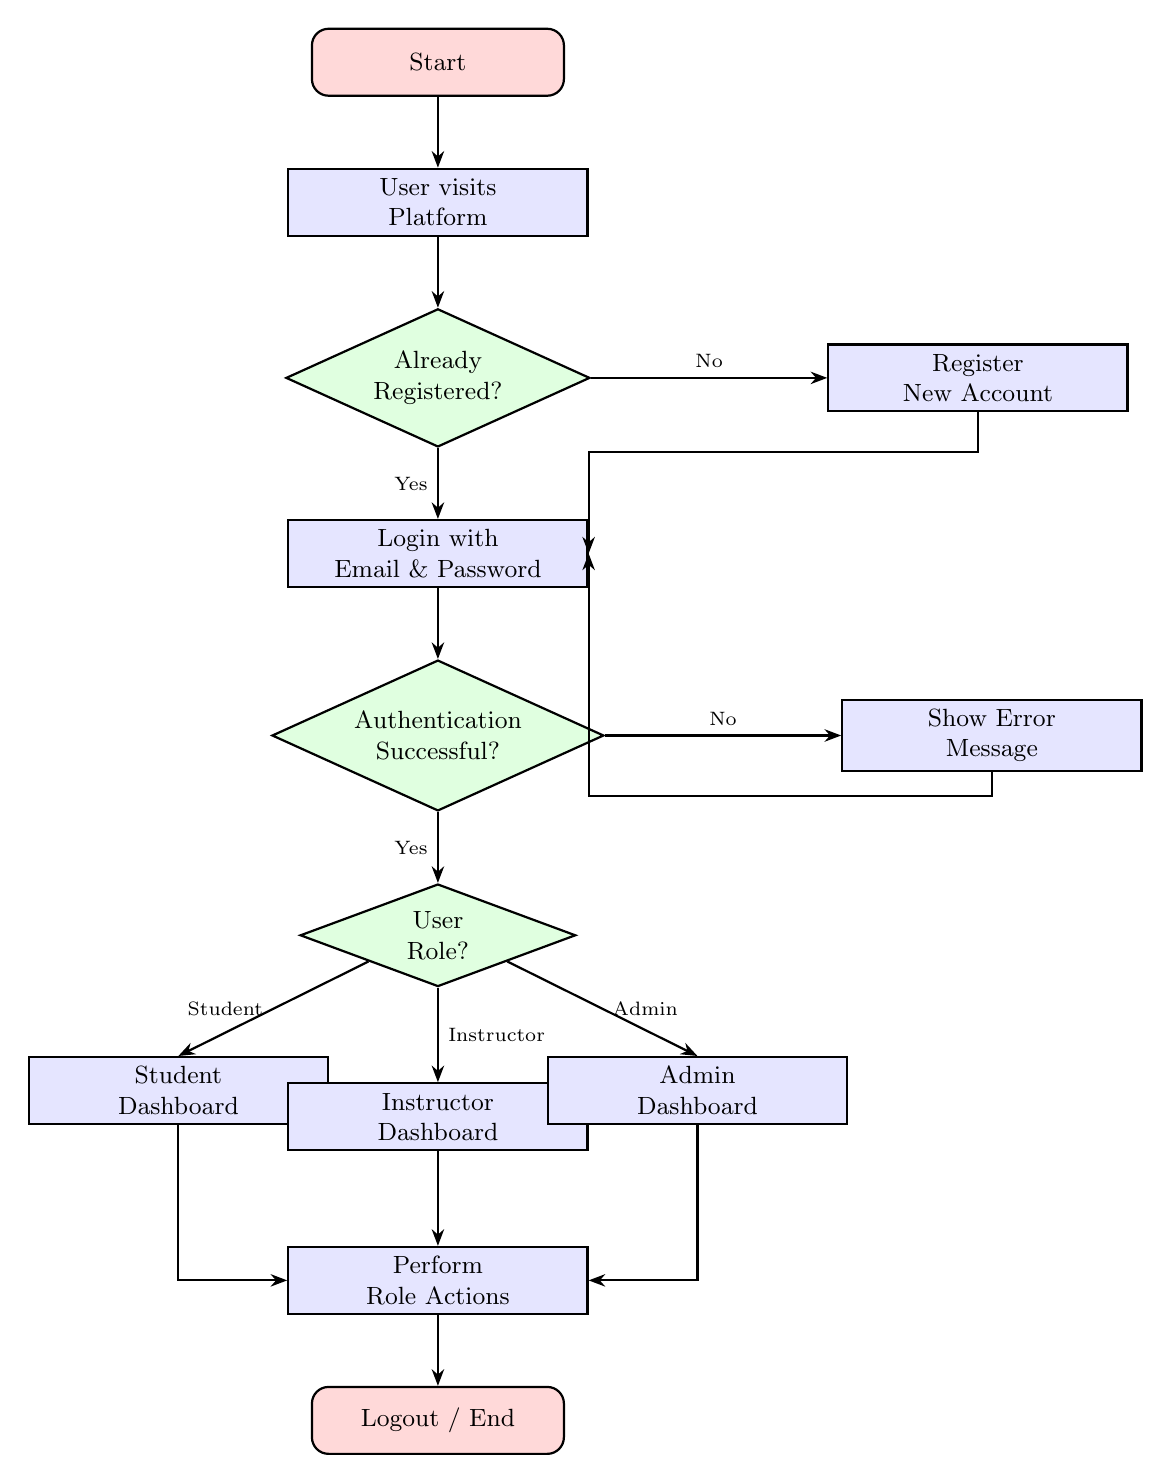
\begin{tikzpicture}[
  node distance = 0.9cm and 3.5cm,   % vertical gap, horizontal gap
  every node/.style = {align=center}
]

% ----- NODES (left column / main flow) -----
\node[startstop]                         (A) {Start};
\node[process,   below=of A]             (B) {User visits\\ Platform};
\node[decision,  below=0.9cm of B]       (C) {Already\\ Registered?};
\node[process,   right=3cm of C]         (D) {Register\\ New Account};
\node[process,   below=0.9cm of C]       (E) {Login with\\ Email \& Password};
\node[decision,  below=0.9cm of E]       (F) {Authentication\\ Successful?};
\node[process,   right=3cm of F]         (G) {Show Error\\ Message};
\node[decision,  below=0.9cm of F]       (H) {User\\ Role?};
\node[process,   below left =1.2cm and 0.5cm of H]  (I) {Student\\ Dashboard};
\node[process,   below       =1.2cm of H]            (J) {Instructor\\ Dashboard};
\node[process,   below right =1.2cm and 0.5cm of H] (K) {Admin\\ Dashboard};
\node[process,   below=1.2cm of J]       (L) {Perform\\ Role Actions};
\node[startstop, below=0.9cm of L]       (M) {Logout / End};

% ----- ARROWS -----
\draw[myarrow] (A) -- (B);
\draw[myarrow] (B) -- (C);

% Yes --> proceed to login
\draw[myarrow] (C) -- node[left,font=\scriptsize]{Yes} (E);

% No --> Register
\draw[myarrow] (C) -- node[above,font=\scriptsize]{No} (D);
% Register loops back to login
\draw[myarrow] (D.south) -- ++(0,-0.5) -| (E.east);

\draw[myarrow] (E) -- (F);

% Auth failed --> Error message
\draw[myarrow] (F) -- node[above,font=\scriptsize]{No} (G);
% Error loops back to login
\draw[myarrow] (G.south) -- ++(0,-0.3) -| (E.east);

% Auth success --> Role check
\draw[myarrow] (F) -- node[left,font=\scriptsize]{Yes} (H);

% Role branches
\draw[myarrow] (H.south west) -- node[left, font=\scriptsize]{Student}     (I.north);
\draw[myarrow] (H.south)      -- node[right,font=\scriptsize]{Instructor}  (J.north);
\draw[myarrow] (H.south east) -- node[right,font=\scriptsize]{Admin}       (K.north);

% All branches converge to Perform Actions
\draw[myarrow] (I.south) |- (L.west);
\draw[myarrow] (J.south)  -- (L.north);
\draw[myarrow] (K.south) |- (L.east);

\draw[myarrow] (L) -- (M);

\end{tikzpicture}
\caption{Flowchart of the Proposed System -- MERN Smart Education Platform}
\label{fig:flowchart}
\end{figure}

\FloatBarrier   % flush all floats before continuing

\subsection{UML Use Case Diagram}

\begin{figure}[H]
\centering
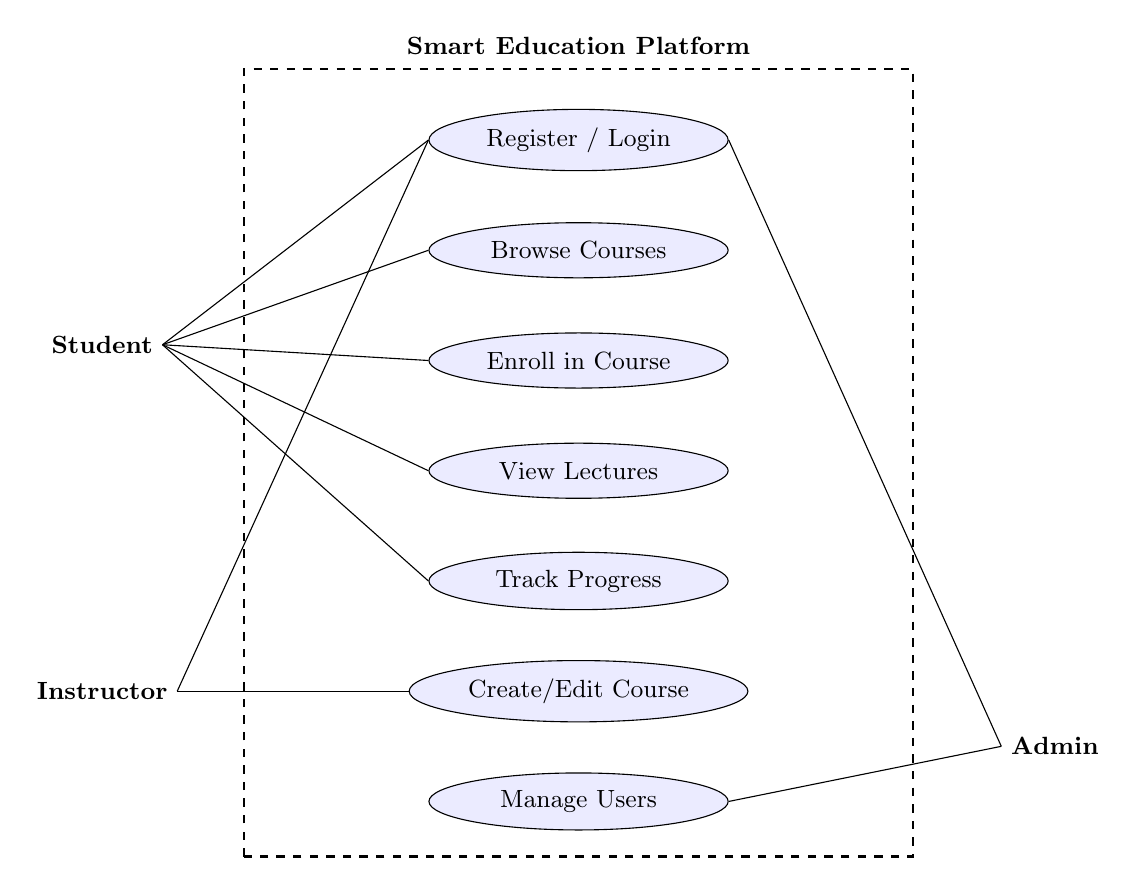
\begin{tikzpicture}[node distance=1.2cm]
  % System boundary
  \draw[thick, dashed] (0,-0.5) rectangle (8.5, 9.5);
  \node[font=\small\bfseries] at (4.25, 9.8) {Smart Education Platform};

  % Use cases inside boundary
  \node[ellipse, draw, fill=blue!8, minimum width=3.8cm, minimum height=0.7cm,
        font=\small, align=center] (uc1) at (4.25, 8.6) {Register / Login};
  \node[ellipse, draw, fill=blue!8, minimum width=3.8cm, minimum height=0.7cm,
        font=\small, align=center] (uc2) at (4.25, 7.2) {Browse Courses};
  \node[ellipse, draw, fill=blue!8, minimum width=3.8cm, minimum height=0.7cm,
        font=\small, align=center] (uc3) at (4.25, 5.8) {Enroll in Course};
  \node[ellipse, draw, fill=blue!8, minimum width=3.8cm, minimum height=0.7cm,
        font=\small, align=center] (uc4) at (4.25, 4.4) {View Lectures};
  \node[ellipse, draw, fill=blue!8, minimum width=3.8cm, minimum height=0.7cm,
        font=\small, align=center] (uc5) at (4.25, 3.0) {Track Progress};
  \node[ellipse, draw, fill=blue!8, minimum width=3.8cm, minimum height=0.7cm,
        font=\small, align=center] (uc6) at (4.25, 1.6) {Create/Edit Course};
  \node[ellipse, draw, fill=blue!8, minimum width=3.8cm, minimum height=0.7cm,
        font=\small, align=center] (uc7) at (4.25, 0.2) {Manage Users};

  % Actors
  \node[font=\small\bfseries] (student)    at (-1.8, 6.0) {Student};
  \node[font=\small\bfseries] (instructor) at (-1.8, 1.6) {Instructor};
  \node[font=\small\bfseries] (admin)      at (10.3, 0.9) {Admin};

  % Student connections
  \draw (student.east) -- (uc1.west);
  \draw (student.east) -- (uc2.west);
  \draw (student.east) -- (uc3.west);
  \draw (student.east) -- (uc4.west);
  \draw (student.east) -- (uc5.west);

  % Instructor connections
  \draw (instructor.east) -- (uc1.west);
  \draw (instructor.east) -- (uc6.west);

  % Admin connections
  \draw (admin.west) -- (uc1.east);
  \draw (admin.west) -- (uc7.east);
\end{tikzpicture}
\caption{UML Use Case Diagram -- Smart Education Platform}
\label{fig:usecase}
\end{figure}

\section{User Interface Design}

The UI is designed using React.js and Tailwind CSS utility classes. All pages share a consistent layout: a fixed top navigation bar for branding and authentication links, a collapsible left sidebar for authenticated dashboard navigation, and a central content pane. The design is fully responsive, adapting gracefully from 320\,px (mobile) through 768\,px (tablet) to 1440\,px (desktop) breakpoints. The primary colour palette is blue (\#3B82F6) and white, with neutral grays for secondary elements, meeting WCAG AA contrast requirements.

\section{Database Design}

\subsection{ER Diagram}

\begin{figure}[H]
\centering
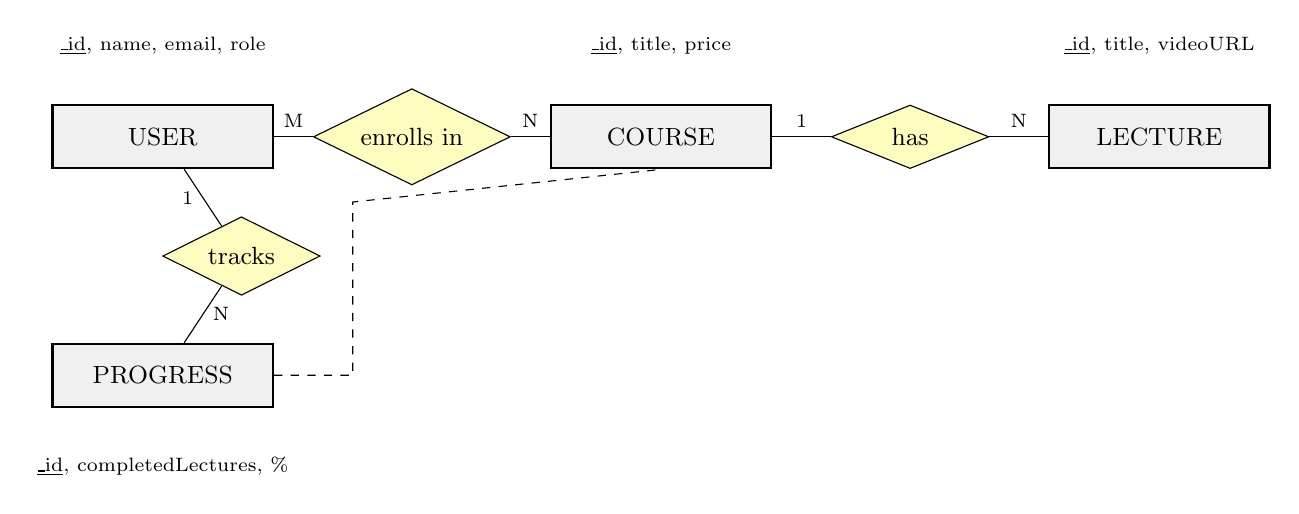
\begin{tikzpicture}[node distance=1.6cm and 3.2cm]
  % Entities
  \node[entity, minimum width=2.8cm] (USER)     {USER};
  \node[entity, minimum width=2.8cm, right=3.5cm of USER]  (COURSE)  {COURSE};
  \node[entity, minimum width=2.8cm, right=3.5cm of COURSE](LECTURE) {LECTURE};
  \node[entity, minimum width=2.8cm, below=2.2cm of USER]  (PROGRESS){PROGRESS};

  % Relationships
  \node[diamond, draw, fill=yellow!25, aspect=2, font=\small,
        minimum width=2.5cm, minimum height=0.8cm]
        (R1) at ($(USER)!0.5!(COURSE)$) {enrolls in};
  \node[diamond, draw, fill=yellow!25, aspect=2, font=\small,
        minimum width=2cm, minimum height=0.8cm]
        (R2) at ($(COURSE)!0.5!(LECTURE)$) {has};
  \node[diamond, draw, fill=yellow!25, aspect=2, font=\small,
        minimum width=2cm, minimum height=0.8cm]
        (R3) at ($(USER)!0.5!(PROGRESS)+(1,0)$) {tracks};

  % Entity-Relationship lines
  \draw (USER)     -- node[above,font=\scriptsize]{M} (R1)
        (R1)       -- node[above,font=\scriptsize]{N} (COURSE);
  \draw (COURSE)   -- node[above,font=\scriptsize]{1} (R2)
        (R2)       -- node[above,font=\scriptsize]{N} (LECTURE);
  \draw (USER)     -- node[left, font=\scriptsize]{1} (R3);
  \draw (R3)       -- node[right,font=\scriptsize]{N} (PROGRESS);
  \draw[dashed] (PROGRESS.east) -- ++(1,0) -- ++(0,2.2) -- (COURSE.south);

  % Key attributes (underlined)
  \node[font=\scriptsize, above=0.5cm of USER]
    {\underline{\_id}, name, email, role};
  \node[font=\scriptsize, above=0.5cm of COURSE]
    {\underline{\_id}, title, price};
  \node[font=\scriptsize, above=0.5cm of LECTURE]
    {\underline{\_id}, title, videoURL};
  \node[font=\scriptsize, below=0.5cm of PROGRESS]
    {\underline{\_id}, completedLectures, \%};
\end{tikzpicture}
\caption{Entity-Relationship Diagram -- Smart Education Platform}
\label{fig:er}
\end{figure}

\FloatBarrier

\subsection{Normalization}

All MongoDB collections are designed in adherence to normalized principles applicable to document-based databases. Each collection stores only attributes belonging to its own entity. Relationships between entities are maintained via ObjectId references rather than embedded documents, thereby preventing data duplication and easing update operations.

\subsection{Database Manipulation}

CRUD operations are performed via Mongoose methods: \texttt{Model.create()}, \texttt{Model.findById()}, \texttt{Model.findByIdAndUpdate()}, and \texttt{Model.findByIdAndDelete()}. Aggregation pipelines are used for computing progress percentages across enrolled courses.

\subsection{Database Connection Controls and Strings}

This structural approach ensures that database connections are managed as a single persistent pool across the lifecycle of the application, eliminating the overhead of opening a new communication pathway for each incoming HTTP request. By specifying optimal parameters such as \texttt{maxPoolSize} and \texttt{serverSelectionTimeoutMS}, the system can automatically scale concurrent database tasks under intense traffic loads. Furthermore, index verification sequences run automatically during this initialization phase to guarantee that search operations maintain sub-second response times. This secure abstraction layer protects the integrity of the data tier while providing transparent telemetry alerts for backend administrators.

\begin{lstlisting}[language=JavaScript, caption={MongoDB Connection Setup (server/config/db.js)}]
import mongoose from 'mongoose';

const connectDB = async () => {
  try {
    await mongoose.connect(process.env.MONGO_URI);
    console.log('MongoDB connected successfully');
  } catch (error) {
    console.error('DB connection error:', error.message);
    process.exit(1);
  }
};

export default connectDB;
\end{lstlisting}

\section{Methodology}

The project adopts the \textbf{Agile methodology} with two-week development sprints. Each sprint began with a planning meeting to define user stories and acceptance criteria, progressed through development and daily self-review, and concluded with a retrospective. Version control was managed using Git with feature branches merged into \texttt{main} only after passing tests. This iterative process ensured continuous improvement and early identification of technical risks.

%%%%%%%%%%%%%%%%%%%%%%%%%%%%%%%%%%%%%%%%%%%%%%%%%%%%%%%%%%%%%%%%%%%%%
%  CHAPTER 4: IMPLEMENTATION, TESTING AND MAINTENANCE
%%%%%%%%%%%%%%%%%%%%%%%%%%%%%%%%%%%%%%%%%%%%%%%%%%%%%%%%%%%%%%%%%%%%%
\chapter{Implementation, Testing and Maintenance}

\section{Introduction to Languages, IDEs, Tools and Technologies Used}

The MERN Smart Education Platform was implemented using the following technologies and tools.

\FloatBarrier
\begin{table}[H]
\centering
\caption{Technologies and Tools Used in the Project}
\label{tab:tech}
\renewcommand{\arraystretch}{1.3}
\begin{tabular}{|p{3.2cm}|p{3.5cm}|p{5.8cm}|}
\hline
\textbf{Category}      & \textbf{Technology}          & \textbf{Purpose} \\
\hline
Frontend               & React.js 18                  & Single Page Application UI \\
\hline
State Management       & Redux Toolkit                & Global client-side state \\
\hline
Styling                & Tailwind CSS                 & Responsive utility-first CSS \\
\hline
Backend                & Node.js + Express.js         & RESTful API server \\
\hline
Database               & MongoDB + Mongoose           & Document storage and ODM \\
\hline
Authentication         & JWT + bcrypt                 & Secure auth and password hashing \\
\hline
IDE                    & Visual Studio Code           & Development environment \\
\hline
API Testing            & Postman                      & Backend endpoint testing \\
\hline
Version Control        & Git + GitHub                 & Source code management \\
\hline
Package Manager        & npm                          & Dependency management \\
\hline
\end{tabular}
\end{table}
\FloatBarrier

\section{Coding Standards of Language Used}

\subsection{JavaScript / Node.js Standards}

\begin{itemize}[leftmargin=1.5cm, itemsep=2pt]
  \item ES6+ syntax including arrow functions, destructuring, and async/await is used throughout the codebase.
  \item Functions follow the single-responsibility principle; each function performs exactly one task.
  \item Variable names use \texttt{camelCase}; constants use \texttt{UPPER\_SNAKE\_CASE}.
  \item All asynchronous functions are wrapped in \texttt{try-catch} blocks with descriptive error messages.
  \item Modules use ES Module syntax (\texttt{import}/\texttt{export}) consistently.
\end{itemize}

\subsection{React Standards}

\begin{itemize}[leftmargin=1.5cm, itemsep=2pt]
  \item All components are functional components using React Hooks (\texttt{useState}, \texttt{useEffect}, \texttt{useSelector}).
  \item Component names follow PascalCase convention.
  \item Props are destructured at the function parameter level for clarity.
  \item Reusable UI components reside in the \texttt{/components} directory; page-level components in \texttt{/pages}.
\end{itemize}

\section{Project Scheduling using GANTT Chart}

\begin{figure}[H]
\centering
\begin{ganttchart}[
  hgrid,
  vgrid = {*{1}{draw=gray!40}},
  x unit = 1.0cm,
  y unit title = 0.65cm,
  y unit chart = 0.55cm,
  title height = 1,
  bar height = 0.5,
  title label font   = \scriptsize,
  bar label font     = \scriptsize,
  group label font   = \scriptsize\bfseries,
  bar/.append style  = {fill=blue!40},
  group/.append style= {fill=blue!70},
]{1}{12}
\gantttitle{Training Period (6 Months)}{12}\\
\gantttitlelist{1,2,3,4,5,6,7,8,9,10,11,12}{1}\\
\ganttgroup{Phase 1: Analysis}{1}{2}\\
\ganttbar{Requirement Gathering}{1}{1}\\
\ganttbar{Feasibility Study}{2}{2}\\
\ganttgroup{Phase 2: Design}{3}{4}\\
\ganttbar{System \& DB Design}{3}{3}\\
\ganttbar{UI Prototyping}{4}{4}\\
\ganttgroup{Phase 3: Implementation}{5}{9}\\
\ganttbar{Backend API (Node/Express)}{5}{7}\\
\ganttbar{Frontend (React/Redux)}{6}{9}\\
\ganttgroup{Phase 4: Testing}{10}{11}\\
\ganttbar{Unit \& Integration Testing}{10}{10}\\
\ganttbar{UAT \& Bug Fixes}{11}{11}\\
\ganttgroup{Phase 5: Documentation}{12}{12}\\
\ganttbar{Report Writing}{12}{12}\\
\end{ganttchart}
\caption{GANTT Chart for Project Development Schedule}
\label{fig:gantt}
\end{figure}

\FloatBarrier

\section{Testing Techniques and Test Plans}

The following testing techniques were applied during the project.

\begin{itemize}[leftmargin=1.5cm, itemsep=2pt]
  \item \textbf{Unit Testing:} Individual controller functions and React components were tested in isolation to verify correct individual behaviour.
  \item \textbf{Integration Testing:} API endpoints were tested end-to-end using Postman to verify correct data flow between the frontend, backend, and database.
  \item \textbf{Black Box Testing:} Testing based solely on expected inputs and outputs, without knowledge of internal implementation logic.
  \item \textbf{User Acceptance Testing (UAT):} A group of test users validated the platform against the defined requirements and reported usability feedback.
\end{itemize}

\section{Test Cases Used in the Project}

\FloatBarrier
\begin{table}[H]
\centering
\caption{Test Cases -- Authentication Module}
\label{tab:tc_auth}
\renewcommand{\arraystretch}{1.3}
\begin{tabular}{|p{0.6cm}|p{3cm}|p{3.2cm}|p{3.2cm}|p{1.3cm}|}
\hline
\textbf{TC\#} & \textbf{Test Case}           & \textbf{Input}                     & \textbf{Expected Output}              & \textbf{Status} \\
\hline
1  & Valid User Login          & Correct email + password           & JWT token set, redirect to dashboard & Pass \\
\hline
2  & Invalid Password          & Correct email + wrong password     & Error: Invalid credentials           & Pass \\
\hline
3  & Empty Fields              & No email, no password              & Validation error displayed           & Pass \\
\hline
4  & New User Registration     & Valid name, email, password        & User created, redirect to login      & Pass \\
\hline
5  & Duplicate Registration    & Already registered email           & Error: User already exists           & Pass \\
\hline
\end{tabular}
\end{table}
\FloatBarrier

\begin{table}[H]
\centering
\caption{Test Cases -- Course Management Module}
\label{tab:tc_course}
\renewcommand{\arraystretch}{1.3}
\begin{tabular}{|p{0.6cm}|p{3cm}|p{3.2cm}|p{3.2cm}|p{1.3cm}|}
\hline
\textbf{TC\#} & \textbf{Test Case}           & \textbf{Input}                     & \textbf{Expected Output}              & \textbf{Status} \\
\hline
6  & Create Course             & Valid course data (instructor)     & Course created and saved in DB       & Pass \\
\hline
7  & Enroll in Course          & Student clicks Enroll button       & Student added to enrolled list       & Pass \\
\hline
8  & Unauthorized Access       & Student accesses instructor route  & 403 Forbidden response returned      & Pass \\
\hline
9  & View Lecture (Enrolled)   & Enrolled student views lecture     & Video / content loads correctly      & Pass \\
\hline
10 & Delete Course             & Instructor deletes own course      & Course removed from database         & Pass \\
\hline
\end{tabular}
\end{table}
\FloatBarrier

%%%%%%%%%%%%%%%%%%%%%%%%%%%%%%%%%%%%%%%%%%%%%%%%%%%%%%%%%%%%%%%%%%%%%
%  CHAPTER 5: RESULTS AND DISCUSSIONS
%%%%%%%%%%%%%%%%%%%%%%%%%%%%%%%%%%%%%%%%%%%%%%%%%%%%%%%%%%%%%%%%%%%%%
\chapter{Results and Discussions}

\section{User Interface Representation}

\subsection{Brief Description of Various Modules of the System}

The MERN Smart Education Platform is organized into the following major functional modules.

\begin{itemize}[leftmargin=1.5cm, itemsep=2pt]
  \item \textbf{Authentication Module:} Handles user registration, login, logout, and JWT session management. Protects all authenticated routes from unauthorized access.
  \item \textbf{Course Management Module:} Allows instructors to create, update, publish, and delete courses along with their associated lecture content.
  \item \textbf{Student Dashboard Module:} Displays enrolled courses with progress bars, provides access to lecture content, and shows course discovery features.
  \item \textbf{Instructor Dashboard Module:} Provides per-course analytics including total enrollment count and published lecture list.
  \item \textbf{Admin Module:} Enables platform-level management of all registered users and all published courses.
  \item \textbf{Progress Tracking Module:} Records each lecture viewed by a student and computes the overall course completion percentage in real time.
  \item \textbf{MCQs:} There are Multiple choice Question Available with Solution for Various Examinations like -- IIT, NEET, Aptitude etc.
  \item \textbf{Free Course and Notes Management: } All these are managed by the Admin itself.
\end{itemize}

\section{Snapshots of System with Brief Detail}

 \begin{figure}[H]
   \centering
   \includegraphics[width=0.88\textwidth]{login_page.png}
   \caption{Login Page -- Smart Education Platform}
   \label{fig:snap_login}
 \end{figure}


% \noindent\textbf{Figure 5.1 -- Login Page}


 \begin{figure}[H]
   \centering
   \includegraphics[width=0.88\textwidth]{sign_up.png}
   \caption{Signup Page – User Authentication Interface}
   \label{fig:snap_login}
 \end{figure}

\noindent The Login Page allows registered users to authenticate using their email address and password. Invalid credentials trigger an inline error message. New users are redirected to the Registration page via the provided link.

\vspace{0.5cm}

% \noindent\textbf{Figure 5.2 -- Student Dashboard}

\begin{figure}[H]
   \centering
   \includegraphics[width=0.88\textwidth]{student_dashboard.png}
   \caption{Student Dashboard – Enrolled Courses and Progress}
   \label{fig:student_dashboard}
 \end{figure}


\noindent The Student Dashboard displays all courses in which the student is enrolled, along with a progress bar for each course showing the percentage of lectures completed.

\vspace{0.5cm}

% \noindent\textbf{Figure 5.3 -- Course Creation (Instructor View)}

\begin{figure}[H]
   \centering
   \includegraphics[width=0.88\textwidth]{course_creation_form.png}
   \caption{Course Creation Form – Instructor Interface}
   \label{fig:course_creation_form}
 \end{figure}


\noindent The Course Creation form allows instructors to provide a title, description, category, thumbnail image, price, and publish status before submitting the course to the platform.

\vspace{0.5cm}

% \noindent\textbf{Figure 5.4 -- Admin Dashboard}

\begin{figure}[H]
   \centering
   \includegraphics[width=0.88\textwidth]{Admin_dashboard.png}
   \caption{Admin Dashboard – User and Course Management}
   \label{fig:Admin_dashboard}
 \end{figure}

\noindent The Admin Dashboard provides a tabular view of all registered users and published courses, with options to remove any entry from the platform.

\section{Back Ends Representation}

\subsection{Snapshots of Database Tables with Brief Description}

% \noindent\textbf{Figure 5.5 -- MongoDB Users Collection}

\begin{figure}[H]
   \centering
   \includegraphics[width=0.88\textwidth]{MongoDb_Collection.png}
   \caption{MongoDB Users Collection – Document Structure}
   \label{fig:MongoDb_Collectionn}
 \end{figure}

\noindent The Users collection stores one document per registered user, including a hashed password, assigned role, profile image URL, and an array of references to enrolled course IDs.

\vspace{0.5cm}

% \noindent\textbf{Figure 5.6 -- MongoDB Courses Collection}

\begin{figure}[H]
   \centering
   \includegraphics[width=0.88\textwidth]{course_Collection.png}
   \caption{MongoDB Courses Collection – Document Structure}
   \label{fig:course_Collection}
 \end{figure}}

\noindent The Courses collection stores course metadata including the instructor's User ObjectId reference, an array of Lecture ObjectId references, and an array of enrolled student ObjectId references.

%%%%%%%%%%%%%%%%%%%%%%%%%%%%%%%%%%%%%%%%%%%%%%%%%%%%%%%%%%%%%%%%%%%%%
%  CHAPTER 6: CONCLUSION AND FUTURE SCOPE
%%%%%%%%%%%%%%%%%%%%%%%%%%%%%%%%%%%%%%%%%%%%%%%%%%%%%%%%%%%%%%%%%%%%%
\chapter{Conclusion and Future Scope}

\section*{Conclusion}
\addcontentsline{toc}{section}{Conclusion}

The MERN Smart Education Platform was successfully designed, developed, and tested over the six months of industrial training. The project demonstrates a complete and functional implementation of a Learning Management System using modern, industry-standard JavaScript technologies across the entire stack. All primary objectives --- user authentication and authorization, course and lecture management, real-time progress tracking, and role-based dashboards --- were achieved within the training period.

Working through the complete Software Development Life Cycle, from requirements analysis and feasibility study through system design, implementation, and testing, provided invaluable practical exposure to real-world software engineering workflows. The technologies employed --- React.js, Node.js, Express.js, and MongoDB --- are among the most widely used in the industry, making the skills acquired through this project directly applicable to professional software development roles.

\section*{Future Scope}
\addcontentsline{toc}{section}{Future Scope}

The following enhancements are identified for future development of the platform.

\begin{itemize}[leftmargin=1.5cm, itemsep=2pt]
  \item \textbf{Payment Integration:} Integration of Razorpay or Stripe to support paid course enrollment and instructor earnings management.
  \item \textbf{Live Sessions:} Implementation of WebRTC-based live video classes enabling real-time interaction between instructors and students.
  \item \textbf{AI-Based Recommendations:} A machine learning recommendation engine to suggest relevant courses based on a student's enrollment history and interests.
  \item \textbf{Mobile Application:} Development of a cross-platform React Native companion application for iOS and Android.
  \item \textbf{Certificate Generation:} Automatic generation and email delivery of PDF completion certificates upon successful course completion.
  \item \textbf{Discussion Forums:} Per-course discussion boards for asynchronous student-instructor interaction and peer learning.
  \item \textbf{Multilingual Support:} Internationalization (i18n) support for regional languages to improve accessibility across diverse student populations.
\end{itemize}

%====================================================================
%  REFERENCES / BIBLIOGRAPHY
%====================================================================
\newpage
\addcontentsline{toc}{chapter}{References}
\begin{center}
{\fontsize{16}{19}\selectfont\bfseries References / Bibliography}
\end{center}
\vspace{0.5cm}

\begin{enumerate}[leftmargin=1.5cm, itemsep=4pt]
  \item Flanagan, D., \textit{JavaScript: The Definitive Guide}, 7th~ed., O'Reilly Media, 2020.
  \item Banks, A.\ \& Porcello, E., \textit{Learning React: Modern Patterns for Developing React Apps}, 2nd~ed., O'Reilly Media, 2020.
  \item Hossain, M.~E., \textit{Node.js Design Patterns}, 3rd~ed., Packt Publishing, 2021.
  \item Sommerville, I., \textit{Software Engineering}, 10th~ed., Pearson Education, 2015.
  \item Pressman, R.~S., \textit{Software Engineering: A Practitioner's Approach}, 8th~ed., McGraw-Hill, 2014.
  \item MongoDB Documentation. [Online]. Available: \url{https://www.mongodb.com/docs/}
  \item React Official Documentation. [Online]. Available: \url{https://react.dev/}
  \item Express.js Documentation. [Online]. Available: \url{https://expressjs.com/}
  \item Mongoose Documentation. [Online]. Available: \url{https://mongoosejs.com/docs/}
  \item JWT Introduction. [Online]. Available: \url{https://jwt.io/introduction/}
  \item Tailwind CSS Documentation. [Online]. Available: \url{https://tailwindcss.com/docs/}
  \item GitHub Repository --- MERN Smart Education Platform. [Online]. Available: \url{https://github.com/jayjaisswal/MERN-Smart-Education-Platform}
\end{enumerate}

%====================================================================
%  ANNEXURES
%====================================================================
\newpage
\addcontentsline{toc}{chapter}{Annexures}
\begin{center}
{\fontsize{16}{19}\selectfont\bfseries Annexures}
\end{center}

\section*{Annexure A: Development Environment}
\addcontentsline{toc}{section}{Annexure A: Development Environment}

\FloatBarrier
\begin{table}[H]
\centering
\caption{Development Environment Specifications}
\label{tab:devenv}
\renewcommand{\arraystretch}{1.3}
\begin{tabular}{|p{4.5cm}|p{8cm}|}
\hline
\textbf{Component}     & \textbf{Specification} \\
\hline
Operating System       & Windows 11  \\
\hline
Code Editor            & Visual Studio Code 1.87+ \\
\hline
Node.js Version        & v18.x LTS \\
\hline
npm Version            & 9.x \\
\hline
Database               & MongoDB Atlas (Cloud) / MongoDB v7.x (Local) \\
\hline
Browser                & Google Chrome v120+ \\
\hline
API Testing Tool       & Postman v10.x \\
\hline
Version Control        & Git v2.40+ \\
\hline
Minimum RAM            & 8\,GB \\
\hline
\end{tabular}
\end{table}
\FloatBarrier

% \section*{Annexure B: Project Directory Structure}
% \addcontentsline{toc}{section}{Annexure B: Project Directory Structure}

% \begin{lstlisting}[caption={Project Directory Structure}]
% MERN-Smart-Education-Platform/
% |-- client/                  # React.js Frontend
% |   |-- src/
% |   |   |-- components/      # Reusable UI components
% |   |   |-- pages/           # Page-level components
% |   |   |-- redux/           # Store, slices, selectors
% |   |   |-- App.jsx          # Root component
% |   |   `-- main.jsx         # Entry point
% |   `-- package.json
% |
% |-- server/                  # Node.js + Express Backend
% |   |-- controllers/         # Route handler functions
% |   |-- models/              # Mongoose schemas & models
% |   |-- routes/              # Express route definitions
% |   |-- middleware/          # Auth & error middleware
% |   |-- config/              # DB connection config
% |   |-- index.js             # Server entry point
% |   `-- package.json
% |
% `-- README.md
% \end{lstlisting}

\end{document}
